\section{Applications}

In the previous sections, we described the goals of various applications
and motivated why it was difficult to accomodate them in the standard
web architecture.  Then, we described the \sys{} system, explaining the
primitives we introduced to the browser.  In this section, we close the
loop, explaining how to use this primitives to implement the
applications described in the first section.

\subsection{Encrypted Document Editor}

In the previous section, we described the key feature needed by an
encrypted document editor: symmetric confinement, where two mutually
distrusting scripts can confine each other's use of data that has been
sent.  The key to implementing this application will be judicious use of
\emph{privileges}, which are asymmetrically distributed to the
distrusting components.

\begin{figure}
\centerline{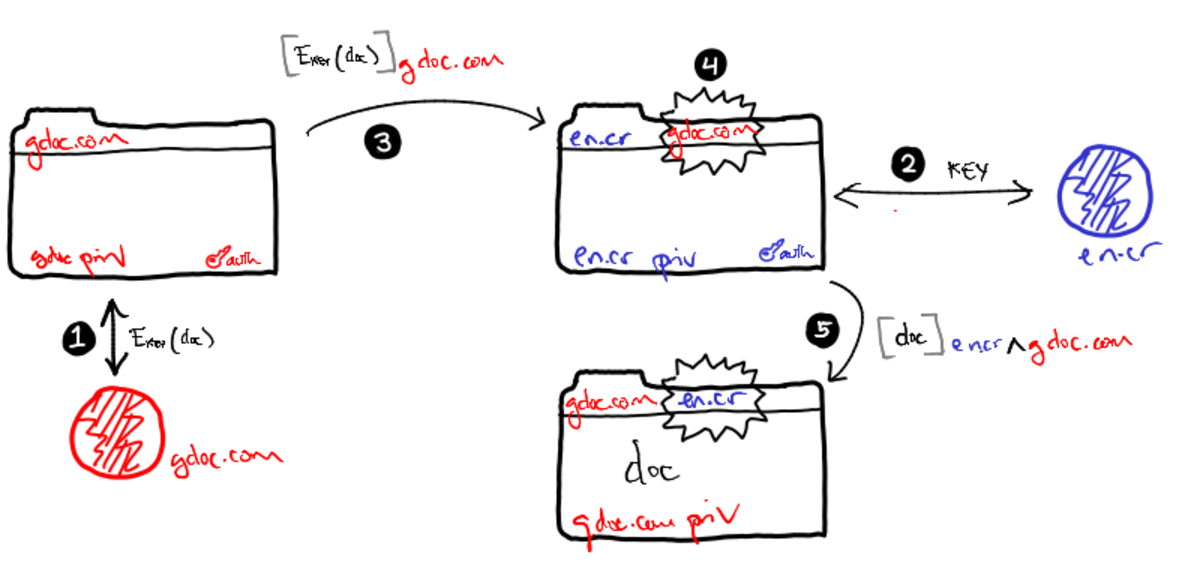
\includegraphics[width=\columnwidth]{editor2-byhand}}
\caption{\label{fig:editor} Encrypted document editor architecture
under \sys{}.}
\end{figure}

In Figure~\ref{fig:editor}, the architecture for \emph{saving a
document} in an encrypted editor editor is shown.  The editor has three
components: a component which has your Google Documents credentials and
communicates with the server, the editor proper, and the component which
performs encryption.  We give the following security guarantee: if the
\https{en.cr} is honest, then we guarantee that the clear text of your document
is never leaked to any origin.  If only \https{gdoc.com} is honest, then
\https{gdoc.com} may be able to recover your cleartext (e.g. the encryptor
used the null cipher), but the encryptor should not able to exfiltrate the
cleartext to anyone else.\footnote{We assume that the user can securely
transmit input to the iframe of their choice---in the face of phishing,
this may not necessarily hold, but we defer this problem for now.}

How does this architecture work when you open an encrypted document?  Initially, only the
first Google Documents window is open, and it downloads (1) the encrypted
document from Google's servers.  When it realizes encryption is needed,
it opens an iframe to \https{en.cr}, exercising its privilege to keep
its initial label as \https{en.cr} so it can (2) talk to the \https{en.cr}
server and download the private key which will be used to decrypt the
document.  (3) Next, it sends the encrypted document as a labeled blob,
with the label ``\https{gdoc.com}''; the iframe raises (4) its label in
order to be able to read and decrypt the document.  Finally, the iframe
passes on the decrypted document (5) to a new iframe which implements the
editor proper, appropriately labeled to ensure that the iframe must raise
its label to ``\https{gdoc.com} and \https{en.cr}'' to read the decryption.

To save the document, we run this flow in reverse: the editor sends a
decrypted document to the encryptor (5), which encrypts it with the
private key.  Then, critically, the encryptor exercises its privileges
to send a labeled blob of the encrypted document which is \emph{only}
labeled \https{gdoc.com} (3).  Since the encryptor is the only compartment
with the \https{en.cr} privilege, all documents must pass through it for
encryption before being sent out to the world; conversely, it itself cannot
exfiltrate any data, as it is operating with \https{gdoc.com} in its label.

One interesting thing to note about this architecture is that a user can
verify that Google Documents appropriately loaded the encryptor, since
without it, it would not be possible to display the decrypted text.  However, when
a new document is being created, the encryptor iframe must be placed
in a separate pop-up window, so that the user can verify that encryption
has been enabled.
